% !TEX root = main.tex

%%%%%%%%%%%%%%%%%%%%%%%%%%%%%%%%%%%%%%%%%%%%%%%%%%%%%%%%%%%%%%%%%%%%%%%%%%%%%%%%%%%%%%%%%%%%%%%%
\section{実験}
%%%%%%%%%%%%%%%%%%%%%%%%%%%%%%%%%%%%%%%%%%%%%%%%%%%%%%%%%%%%%%%%%%%%%%%%%%%%%%%%%%%%%%%%%%%%%%%%
\subsection{F行列の測定方法}
\subsubsection{4端子定数$A,C$の測定}
図3のように回路の接続を行い,$V_1$の絶対値$\left|V_1\right|$ , $V_2$ の絶対値 $\left|V_2\right|$ , $V_{10}$ の絶対値 $\left|V_{10}\right|$ , $V_1$ と $V_2$ の位相差 $\theta_A$ , $V_{10}$ と $V_2$ の位相差 $\theta_C$
をオシロスコープを用いて測定する.$R_{10}$ は電流を求めるための抵抗であり,十分小さい値であることが望ましい.
この実験では $10\,\si{\ohm}$ 程度に設定する.波形が読み取りにくいときは,$R_{10}$ の値を適宜,大きくする.測定結果より

$$
|A|=\frac{\left|V_1\right|}{\left|V_2\right|}
$$
$$
\arg A=\theta_A
$$
$$
|C|=\frac{\frac{\left|V_{10}\right|}{R_{10}}}{\left|V_2\right|}=\frac{\left|V_{10}\right|}{\left|V_2\right| R_{10}}
$$
$$
\arg C=\theta_C \pm \pi
$$

が求められる.
\subsubsection{4端子定数$B,D$の測定}
図4のように回路の接続を行い,$V_1$の絶対値$\left|V_1\right|$ , $V_{10}$ の絶対値 $\left|V_{10}\right|$ , $V_{20}$ の絶対値 $\left|V_{20}\right|$ , $V_1$ と $V_{20}$ の位相差 $\theta_B$ , $V_{10}$ と $V_{20}$ の位相差 $\theta_D$
をオシロスコープを用いて測定する.$R_{10}$,$R_{20}$ は電流を求めるための抵抗であり,十分小さい値であることが望ましい.
この実験では $10\,\si{\ohm}$ 程度に設定する.波形が読み取りにくいときは,$R_{10}$,$R_{20}$ の値を適宜,大きくする.測定結果より

$$
|B|=\frac{\left|V_1\right|}{\frac{\left|V_{20}\right|}{R_{20}}}=\frac{\left|V_1\right| R_{20}}{\left|V_{20}\right|}
$$
$$
\arg B=\theta_B
$$
$$
|D|=\frac{\frac{\left|V_{10}\right|}{R_{10}}}{\frac{\left|V_{20}\right|}{R_{20}}}=\frac{\left|V_{10}\right| R_{20}}{\left|V_{20}\right| R_{10}}
$$
$$
\arg D=\theta_D \pm \pi
$$



\begin{figure}[H]
    \begin{center}
        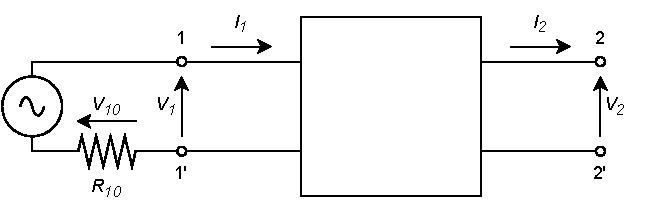
\includegraphics[]{figure3.drawio.pdf}
        \caption{4端子定数$A,C$の測定}
    \end{center}
\end{figure}

\begin{figure}[H]
    \begin{center}
        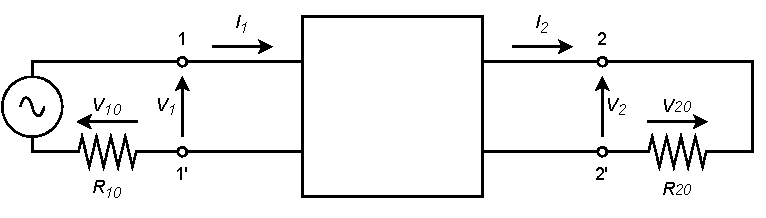
\includegraphics[]{figure4.drawio.pdf}
        \caption{4端子定数$B,D$の測定}
    \end{center}
\end{figure}


\subsection{被測定回路と測定手順}
被測定回路を図$5,6,7$に示す.抵抗,コンデンサの値は $R=1.0\,\si{k\ohm}$ , $C=1.0\,\si{\mu\farad}$ とし,周波数 $f$ は $f=1\,\si{k\hertz}$ とする.
被測定回路 2 は被測定回路 1 の入力端子と出力端子を入れ換えたものである.
また,被測定回路 3 は被測定回路 1 と被測定回路 2 を縦続接続したものである. 以下の順に測定を行う.

\begin{enumerate}
    \item 図5の被測定回路1について,4端子定数$(A_1, B_1, C_1, D_1)$を測定より求める.
    \item 図6の被測定回路2について,4端子定数$(A_2, B_2, C_2, D_2)$を測定より求める.
    \item 図7の被測定回路3について,4端子定数$(A_3, B_3, C_3, D_3)$を測定より求める.
\end{enumerate}

\begin{figure}[H]
    \begin{center}
        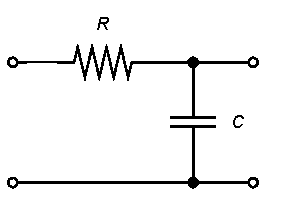
\includegraphics[]{figure5.drawio.pdf}
        \caption{被測定回路1}
    \end{center}
\end{figure}

\begin{figure}[H]
    \begin{center}
        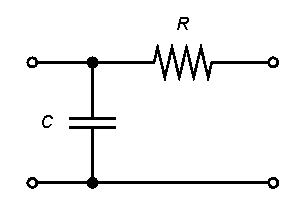
\includegraphics[]{figure6.drawio.pdf}
        \caption{被測定回路2}
    \end{center}
\end{figure}

\begin{figure}[H]
    \begin{center}
        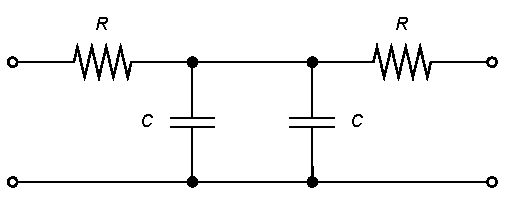
\includegraphics[]{figure7.drawio.pdf}
        \caption{被測定回路3}
    \end{center}
\end{figure}

\subsection{使用機器}
\begin{enumerate}
    \item RC発信機(ケンウッド AG-203A)
    \item DSO(Tektronix TBS1022)
    \item ブレッドボード
\end{enumerate}

\newpage